\documentclass[12pt, a4paper]{article}

\usepackage[utf8]{inputenc}
\usepackage[T1]{fontenc}
\usepackage[brazil]{babel}
\usepackage{lmodern}
\usepackage{geometry}
\usepackage{graphicx}
\usepackage{booktabs}
\usepackage{array}
\usepackage{amsmath}
\usepackage{float}
\usepackage{caption}
\usepackage{parskip}

\geometry{top=2.5cm, bottom=2.5cm, left=2.5cm, right=2.5cm}
\setlength{\parskip}{6pt}

\graphicspath{{../output/}}

\title{\large\textbf{FL Síncrono vs.\ Assíncrono: Comparação entre Datasets}}
\author{Júlio}
\date{\today}

\begin{document}

\maketitle

Este relatório compara o desempenho dos modos síncrono (FedAvg) e assíncrono
(on-the-fly) em três datasets --- MNIST, Fashion-MNIST e CIFAR-10 --- nos cenários
IID e Não-IID, utilizando timeout no percentil~75 (P75) e 5\,000 rodadas/atualizações.

% ─────────────────────────────────────────────
\section{Configuração Experimental}

\begin{table}[H]
\centering
\caption{Parâmetros comuns a todos os experimentos.}
\label{tab:params}
\renewcommand{\arraystretch}{1.25}
\begin{tabular}{lcc}
\toprule
\textbf{Parâmetro} & \textbf{Síncrono} & \textbf{Assíncrono} \\
\midrule
Número de clientes     & 40  & 40  \\
Épocas locais          & 1   & 1   \\
\textit{Batch size}    & 32  & 32  \\
Timeout (percentil)    & P75 & --  \\
$\alpha_0$             & --  & 0{,}8  \\
$\delta$               & --  & 0{,}999 \\
$\lambda$              & --  & 0{,}075 \\
Rodadas / atualizações & 5\,000 & 5\,000 \\
Avaliação a cada       & 10 rodadas/atualizações & 10 atualizações \\
Semente                & 42  & 42  \\
\bottomrule
\end{tabular}
\end{table}

% ─────────────────────────────────────────────
\section{Métricas Utilizadas}

As mesmas métricas são reportadas para todos os datasets e cenários:

\begin{itemize}
    \item \textbf{max\_acc}: acurácia máxima atingida durante o experimento.
    \item \textbf{acc\_final}: acurácia na última avaliação.
    \item \textbf{acc\_at\_5000s}: acurácia no horizonte de 5\,000~s de tempo virtual.
    \item \textbf{loss\_final}: \textit{cross-entropy} na última avaliação.
    \item \textbf{tail\_std}: desvio-padrão das últimas 10 avaliações (estabilidade).
    \item \textbf{time\_to\_90pct\_peak}: tempo virtual (s) para atingir 90\% da acurácia máxima.
    \item \textbf{area\_under\_accuracy\_time}: área integrada sob a curva acurácia $\times$ tempo.
\end{itemize}

% ─────────────────────────────────────────────
\section{CIFAR-10}

\subsection{IID}

\begin{figure}[H]
    \centering
    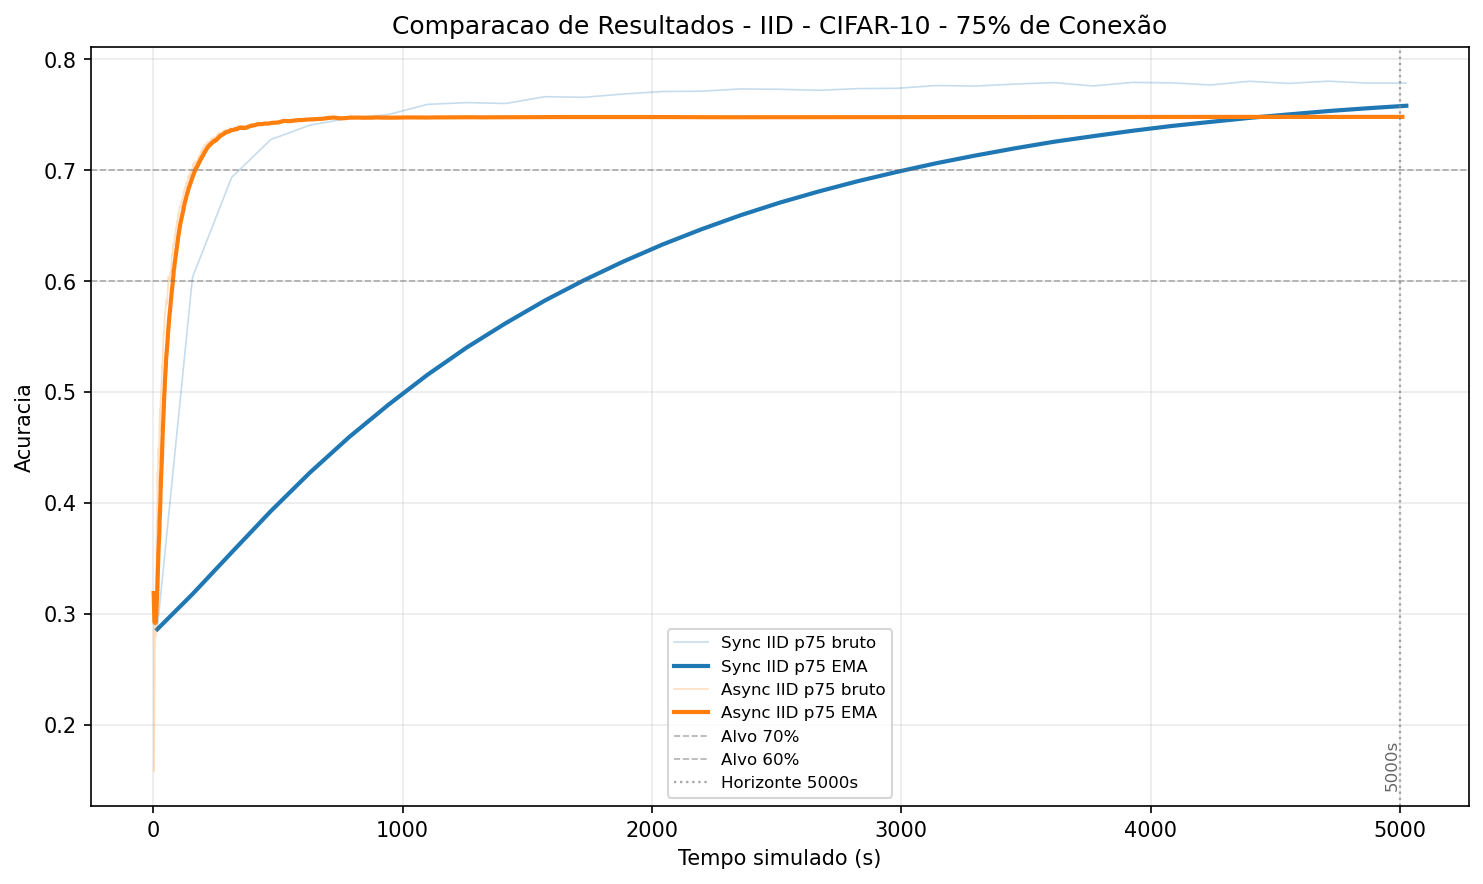
\includegraphics[width=\textwidth]{cifar-10/IID_p75.png}
    \caption{CIFAR-10 / IID --- curvas Sync vs.\ Async.}
\end{figure}

\begin{table}[H]
\centering
\caption{CIFAR-10 --- IID --- Métricas comparativas.}
\label{tab:cifar_iid}
\renewcommand{\arraystretch}{1.25}
\begin{tabular}{lcccccc}
\toprule
\textbf{Métrica} & \textbf{Sync} & \textbf{Async} & \textbf{Vencedor} \\
\midrule
max\_acc           & 0{,}7803 & 0{,}7481 & Sync \\
acc\_final         & 0{,}7786 & 0{,}7481 & Sync \\
acc\_at\_5000s     & 0{,}7786 & 0{,}7481 & Sync \\
loss\_final        & 1{,}0315 & 0{,}7859 & Async \\
tail\_std          & 0{,}0012 & 0{,}0001 & Async \\
time\_to\_90pct\_peak & 471{,}16~s & 116{,}53~s & Async \\
area\_under        & 3781{,}45 & 3715{,}85 & Sync \\
\bottomrule
\end{tabular}
\end{table}

O síncrono atinge acurácia $\approx 3$~p.p.\ superior (78,0\% vs.\ 74,8\%), mas o
assíncrono converge $4{\times}$ mais rápido (116~s vs.\ 471~s) e apresenta perda
final $\approx$ 24\% menor. A área sob a curva é praticamente equivalente.

\subsection{Não-IID}

\begin{figure}[H]
    \centering
    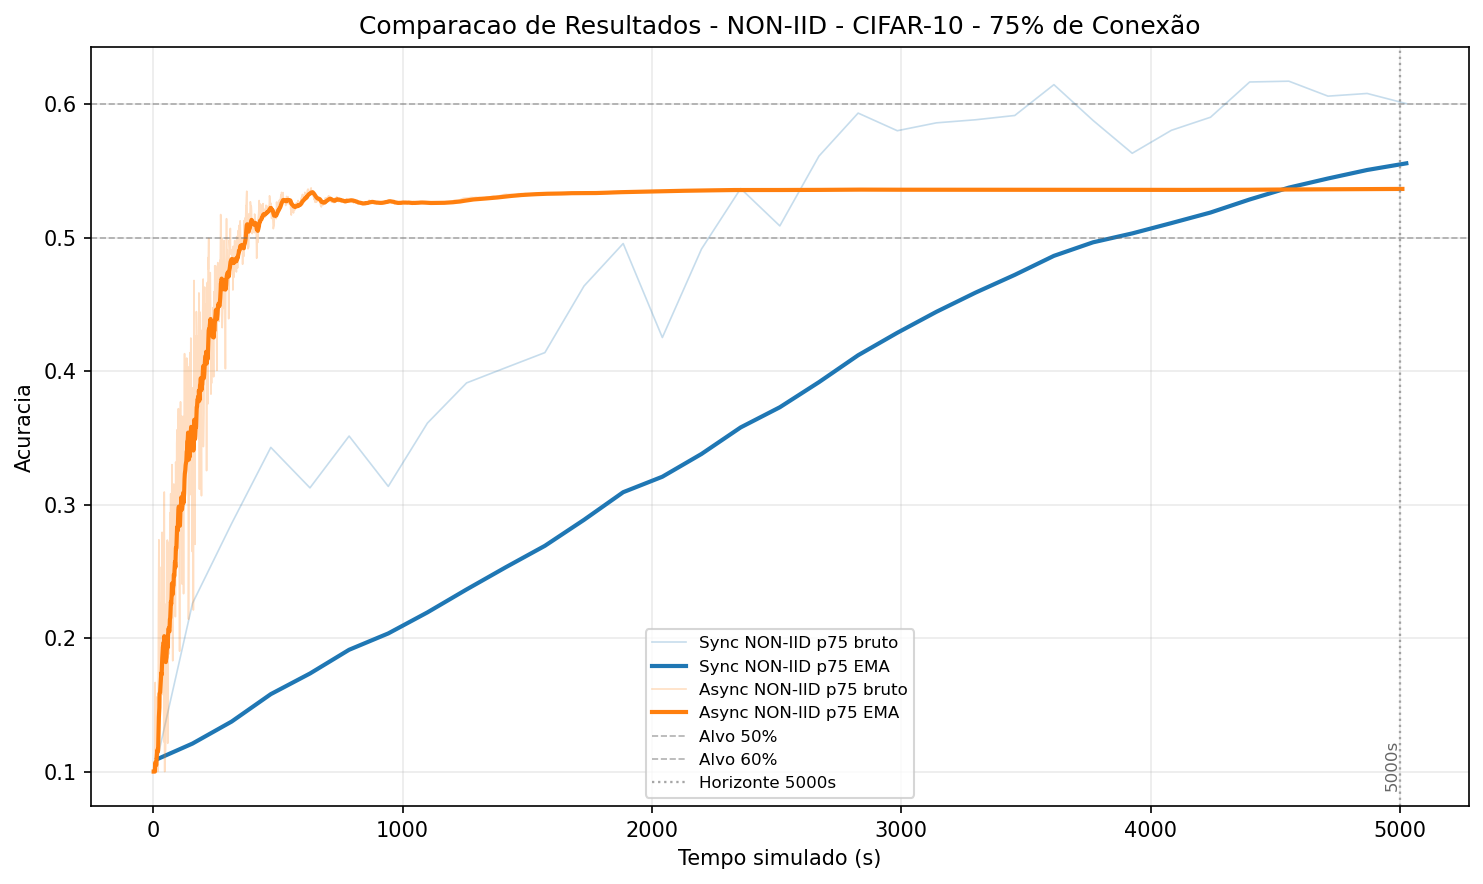
\includegraphics[width=\textwidth]{cifar-10/NON_IID_p75.png}
    \caption{CIFAR-10 / Não-IID --- curvas Sync vs.\ Async.}
\end{figure}

\begin{table}[H]
\centering
\caption{CIFAR-10 --- Não-IID --- Métricas comparativas.}
\label{tab:cifar_noniid}
\renewcommand{\arraystretch}{1.25}
\begin{tabular}{lcccccc}
\toprule
\textbf{Métrica} & \textbf{Sync} & \textbf{Async} & \textbf{Vencedor} \\
\midrule
max\_acc           & 0{,}6171 & 0{,}5372 & Sync \\
acc\_final         & 0{,}6003 & 0{,}5366 & Sync \\
acc\_at\_5000s     & 0{,}6079 & 0{,}5366 & Sync \\
loss\_final        & 1{,}6879 & 1{,}4860 & Async \\
tail\_std          & 0{,}0093 & 0{,}0003 & Async \\
time\_to\_90pct\_peak & 2669{,}91~s & 219{,}60~s & Async \\
area\_under        & 2440{,}98 & 2611{,}35 & Async \\
\bottomrule
\end{tabular}
\end{table}

A vantagem do síncrono em acurácia se amplia em Não-IID ($\approx 8$~p.p.), mas o
assíncrono converge $12{\times}$ mais rápido e é muito mais estável (tail\_std
$32{\times}$ menor). A área integrada favorece o assíncrono, indicando melhor
desempenho acumulado ao longo do tempo.

% ─────────────────────────────────────────────
\section{MNIST}

\subsection{IID}

\begin{figure}[H]
    \centering
    
\includegraphics[width=\textwidth]{mnist/IID_p75.png}
    \caption{MNIST / IID --- curvas Sync vs.\ Async.}
\end{figure}

\begin{table}[H]
\centering
\caption{MNIST --- IID --- Métricas comparativas.}
\label{tab:mnist_iid}
\renewcommand{\arraystretch}{1.25}
\begin{tabular}{lcccccc}
\toprule
\textbf{Métrica} & \textbf{Sync} & \textbf{Async} & \textbf{Vencedor} \\
\midrule
max\_acc           & 0{,}9953 & 0{,}9941 & Sync \\
acc\_final         & 0{,}9953 & 0{,}9937 & Sync \\
acc\_at\_5000s     & 0{,}9953 & 0{,}9937 & Sync \\
loss\_final        & 0{,}0241 & 0{,}0199 & Async \\
tail\_std          & 0{,}0003 & $\approx 0$ & Async \\
time\_to\_90pct\_peak & 15{,}71~s & 1{,}36~s & Async \\
area\_under        & 4975{,}77 & 4990{,}45 & Async \\
\bottomrule
\end{tabular}
\end{table}

Ambos os modos atingem $>99\%$ de acurácia. O assíncrono converge $11{,}6{\times}$
mais rápido e com perda ligeiramente menor, enquanto o síncrono oferece acurácia
marginalmente superior ($+0{,}12$~p.p.), irrelevante na prática para este dataset.

\subsection{Não-IID}

\begin{figure}[H]
    \centering
    
\includegraphics[width=\textwidth]{mnist/NON_IID_p75.png}
    \caption{MNIST / Não-IID --- curvas Sync vs.\ Async.}
\end{figure}

\begin{table}[H]
\centering
\caption{MNIST --- Não-IID --- Métricas comparativas.}
\label{tab:mnist_noniid}
\renewcommand{\arraystretch}{1.25}
\begin{tabular}{lcccccc}
\toprule
\textbf{Métrica} & \textbf{Sync} & \textbf{Async} & \textbf{Vencedor} \\
\midrule
max\_acc           & 0{,}9907 & 0{,}9807 & Sync \\
acc\_final         & 0{,}9881 & 0{,}9807 & Sync \\
acc\_at\_5000s     & 0{,}9902 & 0{,}9807 & Sync \\
loss\_final        & 0{,}0394 & 0{,}0602 & Sync \\
tail\_std          & 0{,}0008 & $\approx 0$ & Async \\
time\_to\_90pct\_peak & 157{,}05~s & 38{,}72~s & Async \\
area\_under        & 4903{,}23 & 4893{,}99 & Sync \\
\bottomrule
\end{tabular}
\end{table}

Em Não-IID, o síncrono retoma vantagem também em perda final. A diferença de
acurácia é de apenas 1~p.p. (99,1\% vs.\ 98,1\%), mas o assíncrono converge
$4{\times}$ mais rápido e permanece praticamente sem oscilações.

% ─────────────────────────────────────────────
\section{Fashion-MNIST}

\subsection{IID}

\begin{figure}[H]
    \centering
    
\includegraphics[width=\textwidth]{fashion-mnist/IID_p75.png}
    \caption{Fashion-MNIST / IID --- curvas Sync vs.\ Async.}
\end{figure}

\begin{table}[H]
\centering
\caption{Fashion-MNIST --- IID --- Métricas comparativas.}
\label{tab:fashion_iid}
\renewcommand{\arraystretch}{1.25}
\begin{tabular}{lcccccc}
\toprule
\textbf{Métrica} & \textbf{Sync} & \textbf{Async} & \textbf{Vencedor} \\
\midrule
max\_acc           & 0{,}9361 & 0{,}9291 & Sync \\
acc\_final         & 0{,}9359 & 0{,}9287 & Sync \\
acc\_at\_5000s     & 0{,}9350 & 0{,}9287 & Sync \\
loss\_final        & 0{,}3224 & 0{,}2136 & Async \\
tail\_std          & 0{,}0010 & $\approx 0$ & Async \\
time\_to\_90pct\_peak & 157{,}05~s & 16{,}57~s & Async \\
area\_under        & 4651{,}00 & 4657{,}22 & Async \\
\bottomrule
\end{tabular}
\end{table}

Padrão consistente com os demais datasets: síncrono ligeiramente superior em
acurácia ($+0{,}7$~p.p.), assíncrono $9{,}5{\times}$ mais rápido e com perda 34\%
menor. A área integrada é praticamente idêntica.

\subsection{Não-IID}

\begin{figure}[H]
    \centering
    
\includegraphics[width=\textwidth]{fashion-mnist/NON_IID_p75.png}
    \caption{Fashion-MNIST / Não-IID --- curvas Sync vs.\ Async.}
\end{figure}

\begin{table}[H]
\centering
\caption{Fashion-MNIST --- Não-IID --- Métricas comparativas.}
\label{tab:fashion_noniid}
\renewcommand{\arraystretch}{1.25}
\begin{tabular}{lcccccc}
\toprule
\textbf{Métrica} & \textbf{Sync} & \textbf{Async} & \textbf{Vencedor} \\
\midrule
max\_acc           & 0{,}8857 & 0{,}8411 & Sync \\
acc\_final         & 0{,}8427 & 0{,}8132 & Sync \\
acc\_at\_5000s     & 0{,}8121 & 0{,}8132 & Async \\
loss\_final        & 0{,}7815 & 0{,}5484 & Async \\
tail\_std          & 0{,}0222 & 0{,}0013 & Async \\
time\_to\_90pct\_peak & 1256{,}43~s & 92{,}37~s & Async \\
area\_under        & 4067{,}94 & 4022{,}19 & Sync \\
\bottomrule
\end{tabular}
\end{table}

O síncrono atinge pico $\approx 4{,}5$~p.p.\ superior, mas sofre queda de $4{,}3$~p.p.\
do pico ao final, enquanto o assíncrono mantém trajetória estável. A acurácia no
horizonte de 5\,000~s é virtualmente idêntica, e o assíncrono converge
$13{,}6{\times}$ mais rápido.

% ─────────────────────────────────────────────
\section{Discussão}

\subsection{Padrões Consistentes}

\begin{enumerate}
    \item \textbf{Acurácia máxima}: o síncrono vence em todos os 6 cenários
    (IID e Não-IID nos 3 datasets). A vantagem é maior em cenários mais difíceis
    (CIFAR-10 Não-IID: $+8{,}0$~p.p.) e menor em datasets simples (MNIST IID:
    $+0{,}12$~p.p.).

    \item \textbf{Velocidade de convergência}: o assíncrono é consistentemente mais
    rápido. O \textit{speedup} varia de $4{\times}$ (CIFAR-10 IID) a $13{,}6{\times}$
    (Fashion-MNIST Não-IID), com mediana de $\approx 10{\times}$.

    \item \textbf{Estabilidade}: o assíncrono apresenta tail\_std ordens de grandeza
    menor em todos os cenários. O síncrono sofre oscilações significativas,
    especialmente em Não-IID (Fashion-MNIST: tail\_std $17{\times}$ maior).

    \item \textbf{Perda final}: o assíncrono vence em 5 de 6 cenários, indicando
    melhor calibração probabilística.

    \item \textbf{Área integrada}: equilíbrio notável --- Sync vence em 3 cenários,
    Async vence em 3. Nenhum modo domina o desempenho acumulado.
\end{enumerate}

\subsection{Impacto da Heterogeneidade (IID $\to$ Não-IID)}

\begin{table}[H]
\centering
\caption{Queda de max\_acc ao passar de IID para Não-IID.}
\label{tab:heterogeneity}
\renewcommand{\arraystretch}{1.25}
\begin{tabular}{lccc}
\toprule
\textbf{Dataset} & \textbf{$\Delta$ Sync} & \textbf{$\Delta$ Async} & \textbf{Assíncrono sofre mais?} \\
\midrule
MNIST         & $-0{,}46$~p.p. & $-1{,}34$~p.p. & Sim ($2{,}9{\times}$) \\
Fashion-MNIST & $-5{,}04$~p.p. & $-8{,}80$~p.p. & Sim ($1{,}7{\times}$) \\
CIFAR-10      & $-16{,}32$~p.p. & $-21{,}09$~p.p. & Sim ($1{,}3{\times}$) \\
\bottomrule
\end{tabular}
\end{table}

Ambos os modos degradam com heterogeneidade, mas o assíncrono sofre queda
proporcionalmente maior em todos os datasets. Isso é esperado: o assíncrono não
sincroniza os modelos locais, acumulando mais \textit{staleness} quando os clientes
têm distribuições enviesadas. Ainda assim, o assíncrono mantém estabilidade superior
mesmo sob heterogeneidade severa.

\subsection{Resumo Geral}

\begin{table}[H]
\centering
\caption{Vitórias por métrica (6 cenários: 3 datasets $\times$ 2 distribuições).}
\label{tab:summary}
\renewcommand{\arraystretch}{1.25}
\begin{tabular}{lcc}
\toprule
\textbf{Métrica} & \textbf{Sync} & \textbf{Async} \\
\midrule
max\_acc             & 6 & 0 \\
acc\_final           & 6 & 0 \\
acc\_at\_5000s       & 5 & 1 \\
loss\_final          & 1 & 5 \\
tail\_std (menor)    & 0 & 6 \\
time\_to\_90pct\_peak & 0 & 6 \\
area\_under          & 3 & 3 \\
\midrule
\textbf{Total}       & 21 & 21 \\
\bottomrule
\end{tabular}
\end{table}

O placar geral é um empate (21--21), o que reflete a natureza complementar dos dois
modos: o síncrono maximiza acurácia absoluta ao custo de tempo e estabilidade; o
assíncrono maximiza eficiência temporal e estabilidade ao custo de acurácia de pico.

A escolha entre os modos deve ser guiada pelo contexto de aplicação: ambientes com
restrição de latência (dispositivos móveis, IoT) beneficiam-se do assíncrono;
aplicações que exigem a maior acurácia possível toleram o custo temporal do síncrono.

\end{document}
